\documentclass[11pt,french,table]{article}
\usepackage[french]{babel}
\usepackage[margin=1in,a4paper]{geometry}

% Custom fonts. This package is only available with XeLaTex (pdflatex is a mess to deal with)
\usepackage{fontspec}
\setmainfont{GeneralSans}[
    Path = assets/fonts/,
    Extension = .otf,
    UprightFont = *-Regular,
    ItalicFont = *-Italic,
    BoldFont = *-Bold,
    BoldItalicFont = *-BoldItalic
]

% Custom titling
\usepackage{titling}
\usepackage{tcolorbox}

% Lipsum paragraphs
\usepackage{lipsum}

% Custom headers
\usepackage{fancyhdr}
\pagestyle{fancy}
\fancyhead[L]{\theauthor}
\fancyhead[C]{\itshape{\thetitle}}
\fancyhead[R]{\thedate}
\setlength{\headheight}{15pt}

% Default mathematical packages
\usepackage{amsmath}
\usepackage{amsfonts}
\usepackage{multicol}

% Exercises environment and styling
\usepackage{amsthm}
\newtheoremstyle{exercice}%
    {3pt}% Space above
    {3pt}% Space below
    {\large}% Body font
    {}% Indent amount
    {\bfseries}% Theorem head font
    {.}% Punctuation after theorem heading
    {\newline}% Space after theorem heading
    {\thmname{#1}\thmnumber{ #2}\thmnote{: #3}}% Theorem head spec (can be left empty, meaning ‘normal’)
\theoremstyle{exercice}
\newtheorem{exercice}{Exercice}
\newtheoremstyle{corrigé}%
    {3pt}% Space above
    {3pt}% Space below
    {\large}% Body font
    {}% Indent amount
    {\bfseries}% Theorem head font
    {.}% Punctuation after theorem heading
    {\newline}% Space after theorem heading
    {\thmname{#1}\thmnumber{ #2}\thmnote{: #3}}% Theorem head spec (can be left empty, meaning ‘normal’)
\theoremstyle{corrigé}
\newtheorem{corrigé}{Corrigé}

% Graphics
\usepackage{graphicx}

\pretitle{\begin{center}\LARGE\bfseries}
\title{Analyse Avancée I - Corrigé II}
\posttitle{\par\end{center}}

\renewcommand{\maketitlehookb}{
\begin{center}
\includegraphics[width=2cm]{assets/imgs/S4S_logo.png}
\end{center}
}

\author{Students 4 Students}
\date{Septembre 2022}

\renewcommand{\maketitlehookd}{
\begin{center}
\begin{tcolorbox}[boxrule=0pt,frame empty,width=0.8\textwidth]
La pensée mathématique est belle parce qu'elle est possible n'importe où.
\end{tcolorbox}
\scriptsize{Cette série vous est délivrée par Lounès, Louis et Till.} 
\end{center}
}

\begin{document}

\maketitle
\begin{corrigé}
      

    Pour $n$ allant de $0$ à $4$, il vient que 
     \begin{multicols}{2}
    \begin{enumerate}
   
        \item[(a)] $a_n=(1,\frac{1}{4},\frac{1}{7},\frac{1}{10},\frac{1}{13})$
        \item[(b)] $b_n=(-1,\frac{4}{3},1,\frac{10}{13},\frac{13}{15})$
   
    \columnbreak  % uniquement si tu veux changer de colonne à un endroit précis
    \item[(c)] $c_n=(0,\frac{1}{3},\frac{2}{9},\frac{3}{27},\frac{4}{81})$. 
     \end{enumerate}
\end{multicols}
(d)
    $d_n = (\sin{(0)},\sin{(\frac{\pi}{4})},\sin{(\frac{2\pi}{4})}, \sin{(\frac{3\pi}{4})},\sin{(\frac{4\pi}{4})})=(0,\frac{\sqrt{2}}{2},1,\frac{\sqrt{2}}{2},0)$. \\
    
Pour la suite $c_n$, le premier terme pour $n=0$ donne bien 0. En effet n'importe quel nombre à la puissance 0 donne 1. Donc pour $n=0$ on a $\frac{0}{3^0}=\frac{0}{1}=0$, cette suite est bien définie pour tout $n\in \mathbb{N}$.
\end{corrigé}
\vspace{1em}
\begin{corrigé}
      Pour cet exercice plusieurs approches sont possibles. En factorisant toujours par la plus grande puissance de $n$ et en utilisant que pour tout $a\in \mathbb{R}$, $\lim\limits_{n\to \infty}{\frac{a}{n}}=0$, nous avons 
    \begin{enumerate}
   
        \item[(a)] $\lim\limits_{n\to \infty}{a_n}=\lim\limits_{n\to \infty}{\underbrace{\frac{1}{n}}_{=0}\underbrace{\frac{1}{3+1/n}}_{=1/3}}=0$. La suite converge donc vers $0$.
        \item[(b)] $\lim\limits_{n\to \infty}{b_n}=\lim\limits_{n\to \infty}{\frac{n}{n}\frac{3+1/n}{4-1/n}}=\frac{3}{4}.$ La suite converge vers $\frac{3}{4}.$
        
         \item[(c)] Pour cette suite nous n'avons pas de preuve rigoureuse mais on peut essayer avec un calculateur graphique de deviner son comportement. On voit alors que la suite converge vers 0 à cause de la croissance exponentielle de $3^n$ par rapport à $n$.
    
    $\lim\limits_{n\to \infty}{c_n}=\lim\limits_{n\to \infty}{\frac{n}{3^n}}=0$. La suite converge vers 0.  
    \begin{figure}[h!]
        \centering
        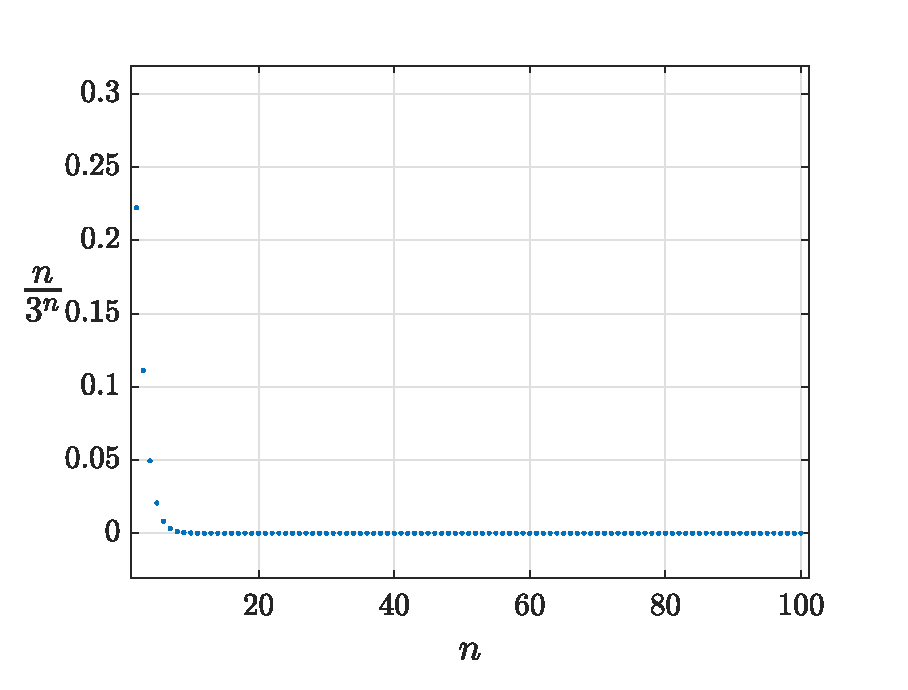
\includegraphics[width=90mm]{exp.eps}
        \caption{Croissance exponentielle qui domine la croissance linéaire, exercice $2-c)$.}
        \label{fig:my_label}
    \end{figure}
    \item[(d)] Sur n'importe quel intervalle de longueur $2\pi $ la fonction prendra toute les valeurs entre $-1$ et $-1$. La fonction ne peut donc converger. 
    \end{enumerate}
\end{corrigé}
\vspace{1em}
\begin{corrigé}
      On suit le même protocole que pour l'exercice précédent. 
    \begin{multicols}{3}
    \begin{enumerate}
   
        \item[(a)] $\lim\limits_{n\to \infty}{a_n}=1$
        \item[(b)] $\lim\limits_{n\to \infty}{b_n}=1$
   \item[(c)] $\lim\limits_{n\to \infty}{c_n}=\lim\limits_{n\to \infty}{\frac{1}{2^n}}=0$
   \item[(d)] $\lim\limits_{n\to \infty}{d_n}=1+0=1$
    \item[(e)] $\lim\limits_{n\to \infty}{e_n}=\text{diverge}$
    \columnbreak  
    \item[(f)] $\lim\limits_{n\to \infty}{f_n}=0$
    \item[(g)] $\lim\limits_{n\to \infty}{g_n}=\infty$
    \item[(h)] $\lim\limits_{n\to \infty}{h_n}=\text{diverge}$
     \item[(i)] $\lim\limits_{n\to \infty}{i_n}=0$
    \item[(j)] $\lim\limits_{n\to \infty}{j_n}=\frac{7}{2}$
    \columnbreak 
    \item[(k)] $\lim\limits_{n\to \infty}{k_n}=\infty$
    \item[(l)] $\lim\limits_{n\to \infty}{l_n}=$diverge
      \item[(m)] $\lim\limits_{n\to \infty}{m_n}=\infty$
      \item[(n)] $\lim\limits_{n\to \infty}{n_n}=0$
      \item[(o)] $\lim\limits_{n\to \infty}{o_n}=0$
      \item[(p)] $\lim\limits_{n\to \infty}{p_n}=0$
      \columnbreak 
     \end{enumerate}
     \end{multicols}
     Pour la suite $o_n$ il faut remarquer que l'on peut appliquer les gendarmes avec l'inégalité : $0<\frac{3^n}{n!}=1 \cdot 3 \cdot \frac{3}{2} \cdot \frac{3}{3} \cdot \frac{3}{4} ... \cdot \frac{3}{n} < \frac{9}{2} \cdot \frac{3}{n} \xrightarrow[]{} 0$
\end{corrigé}
\vspace{1em}
\begin{corrigé}
\begin{enumerate}
    \item[(a)] En utilisant l'indication, on a $\lim\limits_{n  \to \infty}{x_n}=0$. \\  
    \item[(b)] $\sqrt{n^2+n}-n=\frac{(\sqrt{n^2+n}-n)(\sqrt{n^2+n}+n)}{\sqrt{n^2+n}+n}$. En utilisant l'identité $a^2-b^2=(a+b)(a-b)$, on obtient $ \frac{n}{\sqrt{n^2+n}+n}$, et donc $\lim\limits_{n  \to \infty}{\sqrt{n^2+n}-n}=1/2$.
    \item[(c)] $\sqrt{4n^2+n}-2n=\frac{n}{\sqrt{4n^2+n}+2n}$, et donc $\lim\limits_{n  \to \infty}{\sqrt{4n^2+n}-2n}=1/4$
    \end{enumerate}
\end{corrigé}
\vspace{1em}
\begin{corrigé}
\textit{Discussion}. Pour cet exercice, il est important de bien maîtriser la différence entre un nombre irrationnel (c'est-à-dire  qui appartient à $\mathbb{R}/\mathbb{Q}$) et un nombre rationnel (c'est-à-dire qui appartient à $\mathbb{Q}$). Pour rappel, la définition d'un nombre rationnel est un nombre qui peut s'exprimer sous la forme $\frac{n}{1}$ avec $n\in \mathbb{Z}, \ l \in \mathbb{N}$. \\
Chaque nombre rationnel peut s'écrire d'une infinité de manières différentes sous forme de fraction, par exemple : $1/2=2/4=3/6=\cdots$. De plus comme tous les réels, les rationnels admettent une représentation en développement décimal illimité. Le développement décimal des nombres rationnels a la particularité d'être périodique ou finis : $1/3=0,33333333333\cdots$.\\ Notez finalement que $\sqrt{2}$ est irrationnel.\\
\begin{enumerate}
    \item[(a)] Pour le premier cas de figure on veut une suite qui a des valeurs irrationnels mais qui converge vers un rationnel donc un nombre qui peut s'écrire sous forme de fraction, dont le numérateur et le dénominateur sont premiers entre eux. La suite $x_n=\frac{\sqrt{2}}{n}+1$ est constituée de nombres irrationnels ayant pour limite $\lim\limits_{n\to \infty}{x_n}=1$ qui est rationnel.
    \item[(b)] C'est l'inverse cette fois-ci. La suite $r_n=(1+ 1/n)^n$ est constituée de nombres rationnels et a une limite $\lim\limits_{n\to \infty}{r_n}=e$. 
\end{enumerate}
\end{corrigé}
\vspace{1em}
\begin{corrigé}
\begin{enumerate}
    \item[(i)]  Soit $(x_n)$ une suite, alors $(x_n)$ converge vers une limite $ \ l \in \mathbb{R}$ si et seuleument si $\forall \epsilon > 0, \ \exists  \ N \in \mathbb{N} \ \text{tel que } \forall n>N, \ \lvert x_n - l \lvert <\epsilon$.\item[]
    \item[(ii)] 
    \begin{enumerate}
       \item[(a)]
  \textit{Discussion}. Notre tâche est de considérer un $\epsilon>0$ arbitraire et de montrer
qu'il existe un nombre $N$ [qui dépendra de $\epsilon$] tel que $n > N$ implique $|\frac{1}{n^2}-0|<\epsilon$. Nous nous attendons donc à ce que notre preuve formelle commence par 
   "Soit $\epsilon >0$" et qu'elle se termine par quelque chose comme "Donc $n > N$ implique $|\frac{1}{n^2}-0|<\epsilon$". Entre les deux, la preuve devrait spécifier un $N$ et ensuite
vérifier que $N$ a la propriété désirée, à savoir que $n > N$ implique effectivement $|\frac{1}{n^2}-0|<\epsilon$. 
 Dans cet exemple, nous voulons $|\frac{1}{n^2}-0|<\epsilon$ et nous voulons savoir quelle doit être la taille de $n$.\\ Nous allons donc opérer sur cette inégalité algébriquement et essayer de "résoudre" pour $n$. Nous voulons donc $\frac{1}{n^2}<\epsilon$. En multipliant les deux côtés par $n^2$ et
 en divisant les deux côtés par $\epsilon$,nous voulons que finalement que $1/\sqrt{\epsilon}<n$. Si nos
   étapes sont réversibles, on voit que $n>1$ implique $|\frac{1}{n^2}-0|<\epsilon$. Ceci suggère que nous devons prendre $N=\frac{1}{\sqrt{\epsilon}}$.
\paragraph{Preuve Formelle}
Soit $\epsilon>0$. Soit ensuite $N=\frac{1}{\sqrt{\epsilon}}$. Alors $n>N$ implique que $n>\frac{1}{\sqrt{\epsilon}}$ ce qui implique par succession que $\epsilon>\frac{1}{n^2}$. Ainsi en particulier, $n>N$ implique $|\frac{1}{n^2}-0|<\epsilon$. Ceci prouve $\lim \frac{1}{n^2}=0$. \flushright $\Box$ \flushleft
\item[(b)]
Ici pour trouver le rang $N$ le mieux est de majorer pour avoir quelque chose de plus simple : 
\begin{align*}
    \bigg|\frac{4n^3+3n}{n^3-6}-4 \bigg|=\bigg|\frac{3n+24}{n^3-6} \bigg|<\bigg|\frac{3n+24}{(1/2)n^3} \bigg|\leq\bigg|\frac{6}{n^2} \bigg|+\bigg|\frac{48}{n^3} \bigg|
\end{align*}
Si le dernier termes de l'inégalité est plus petit que $\epsilon$ alors on aura bien $$\bigg|\frac{4n^3+3n}{n^3-6}-4 \bigg|<\epsilon.$$ \\ De manière indépendante on a : 
\begin{align*}
    \bigg|\frac{6}{n^2} \bigg|<\frac{\epsilon}{2}
    \Longleftrightarrow n>\frac{12}{\sqrt{\epsilon}} \\
    \bigg|\frac{48}{n^3} \bigg|<\frac{\epsilon}{2} \Longleftrightarrow n>\frac{96}{\sqrt[3]{\epsilon}}
\end{align*}
En posant $N=\max\{\frac{6}{\sqrt{\epsilon}},\frac{48}{\sqrt[3]{\epsilon}}\}$ on obtient bien $\bigg|\frac{4n^3+3n}{n^3-6}-4 \bigg|<\frac{\epsilon}{2}+\frac{\epsilon}{2}=\epsilon$. 
  \end{enumerate}
  \item[(c)] \textit{Discussion}. Nous allons supposer que lim$(-1)^n=l$ et obtenir une contradiction. Quelle que soit la valeur de $l$, soit 1, soit $-1$ aura une distance d'au moins 1 de $l$. Ainsi, l'inégalité $|(-1)^n-l| < 1$ ne sera pas valable pour toutes les grandes valeurs de $n$.
\paragraph{Preuve formelle}
Supposons lim$(-1)^n=l$ pour un certain $l\in \mathbb{R}$. En laissant $\epsilon=1$ dans la définition de la limite, on voit qu'il existe $N_\epsilon$ tel que $n > N_\epsilon$ implique $|(-1)^n-l| < 1$.
En considérant à la fois un $n > N$ pair et impair, on voit que
$$|1-l|<1 \text{ et } |-1-l|<1.$$
\\
Maintenant par l'inégalité triangulaire, il vient \begin{equation*}
   2 = |1-(-1)| = |1-l+l-(-1)| \leq |1-l|+|l-(-1)| < 1+1 = 2. 
\end{equation*}

Cette absurdité montre que notre hypothèse lim$(-1)^n =l$ doit être fausse, donc la suite $(-1)^n$ ne converge pas. \flushright $\Box$
\flushleft
    \end{enumerate}



\end{corrigé}
\vspace{1em}
\begin{corrigé}
   On suit l'indication. On regarde l'inégalité suivante et on la modifie pour faire apparaître des définitions que nous connaissons  : 
    \begin{equation*}
        \begin{aligned}
            |x_ny_n-xy| &= |x_ny_n-x_ny+x_ny-xy| \\ 
        &\leq |x_ny_n-x_ny|+|x_ny-xy|=|x_n|\cdot |y_n-y|+|y|\cdot |x_n-x|.
        \end{aligned}
    \end{equation*}
    Pour de grands $n$, $|y_n-y|$ et $|x_n-x|$ sont petits (définition de convergence) et $|y|$ est bien évidemment constant. 
    Il nous reste à connaître la nature de $|x_n|$. On utilise le fait que \textbf{toute suite convergente est bornée !} Donc $|x_n|$ est bornée par un certain $C\in \mathbb{R}$ et donc il est simple de montrer que $|x_ny_n-xy|$ est petits pour de grands $n$. 
\end{corrigé}
\end{document}